\subsection{Instructor Stakeholders}
\label{sec:instructor_stakeholders}

Instructors are a second group of stakeholders that can benefit from
the easy interpretability of our course sequence visualizations. It is
of particular interest to instructors to gain an overview of the sorts
of students enrolling in their courses, in order to customize
and improve lesson plans \cite{Leaver2002}.

\begin{figure}[h]
    \centering
    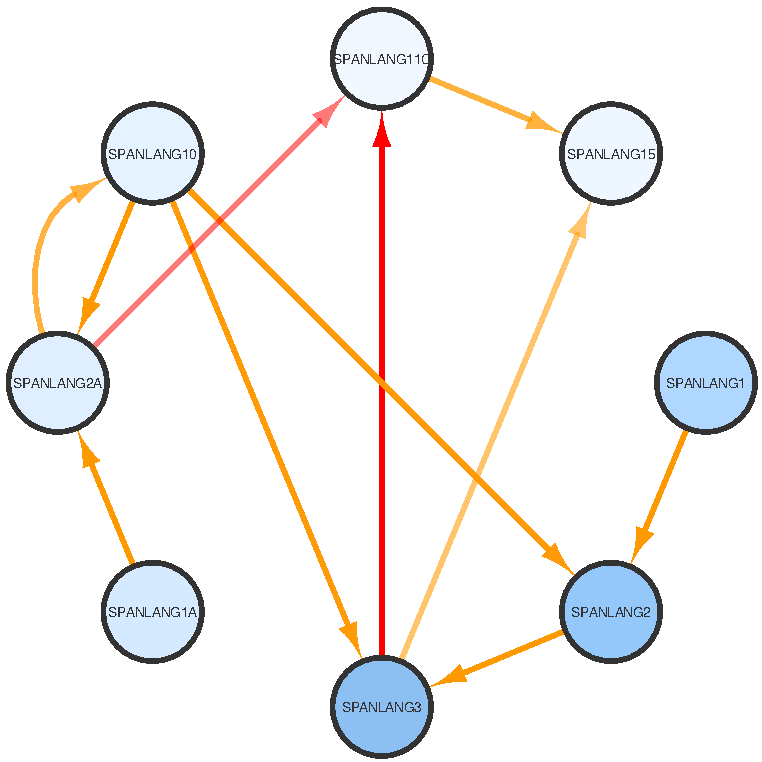
\includegraphics[width=0.4\columnwidth]{Figs/final-spanlang.pdf}  
    \caption{Relationships within the language department's Spanish course offerings from 2012-2016. We note that the probability that a student transitions from first to second year Spanish significantly increases if initially enrolled in the non-accelerated track.}
    \label{fig:spanlang}
\end{figure}

As an example, we show that it is possible to use the course probabilities associated with course-to-course interactions to study the background of students who take higher-level Spanish language classes. We do this by examining the conditional probability graph generated with
all enrollment data. We set our function $d$ as sensitive only to
enrollments in course pairs within one year of each other in order to
capture delayed enrollment behaviors. We can thus interpret edge
weights as probability $p(i|j \text{ within the past year})$. In
Figure~\ref{fig:spanlang}, we examine the courses associated with the
V-structure colored in red---\textsc{spanlang3} (bottom),
\textsc{spanlang2a} (left), and \textsc{spanlang11c}
(top). \textsc{spanlang3} is the final term of the non-accelerated
offering of the first-year Spanish language sequence,
\textsc{spanlang2a} is the final term of the accelerated first-year
sequence (often taken by students with prior exposure to the language
through high school programs), and \textsc{spanlang11c} is the first
academic term of the second-year sequence.

From the visualization alone, it is evident that the relationship
between \textsc{spanlang3} and \textsc{spanlang11c} is stronger than
the relationship between \textsc{spanlang2a} and
\textsc{spanlang11c}. Indeed, the probability that a student enrolls
in \textsc{spanlang11c} within a year of completing \textsc{spanlang3}
is almost three times that of a student who enrolls in
\textsc{spanlang11c} after completing \textsc{spanlang2a}, with
$p(\textsc{spanlang11c}|\textsc{spanlang3}) = 0.038$ and
$p(\textsc{spanlang11c}|\textsc{spanlang2a}) = 0.013$.

This information is not readily gleaned from standard enrollment
figures. The number of students enrolled in \textsc{spanlang11c}
during the graph's time period is almost identical to enrollment in
\textsc{spanlang2a}. One might be erroneously tempted from these
numbers alone to conclude that most {\em 2a} students move on to
\textsc{spanlang11c}. Accounts based on raw enrollment are further
complicated by the observation that enrollment in \textsc{spanlang1-3}
is non-monotonic, first falling, then rising. The cause is
likely that students enroll in \textsc{spanlang3} directly.

A large contribution to \textsc{spanlang11c} beyond \textsc{spanlang3}
are in fact not {\em 2a} students, but students who are already
proficient enough to engage this culture-oriented class directly.

{\em Via} does not help an analysis of underlying reasons for
preferences between the two Spanish language sequences. However,
learning literature does suggest a reason. The observation is in
accordance with the research of Leaver \textit{et al.}, which details
the significance of varying teaching philosophies commonly seen in
foreign language classrooms at different language acquisition levels
\cite{Leaver2002}.

It is possible that the preference for the \textsc{spanlang1-3}
sequence is explained by the difference between instruction of
grammatical foundations in the university's introductory courses
compared to high school language programs.

We next describe details of how we construct the graphs in the above
applications from raw enrollment data.
